\section{Dữ liệu 3}

Bộ dữ liệu ghi lại tỷ lệ tai nạn, gồm 39 quan trắc được thực hiện trên vài đoạn đường cao tốc ở tiểu bang Minnesota vùng Trung Tây của Hoa Kỳ.

\subsection*{Tìm hiểu dữ liệu}

Bộ dữ liệu gồm 13 biến sau:
\begin{itemize}[label=--]
	\item $Y$ : tỷ lệ \% tai nạn trên đoạn đường khảo sát.
	\item $X1$ : chiều dài đoạn đường (dặm).
	\item $X2$ : lượng giao thông trung bình hàng ngày (nghìn xe).
	\item $X3$ : tỷ lệ \% xe tải trên tổng số.
	\item $X4$ : tốc độ giới hạn cho phép (dặm/giờ).
	\item $X5$ : chiều rộng làn đường (bước chân).
	\item $X6$ : chiều rộng làn đường khẩn cấp (bước chân).
	\item $X7$ : số làn đường thay đổi tự do trên đoạn đường cao tốc.
	\item $X8$ : số làn đường thay đổi (báo hiệu) trên đoạn đường cao tốc.
	\item $X9$ : số cửa vào đoạn đường cao tốc.
	\item $X10$ : tổng số làn đường (trên hai chiều của đường cao tốc).
	\item $X11$ : 1 nếu là tuyến đường liên thông xa lộ và cao tốc, 0 nếu ngược lại.
	\item $X12$ : 1 nếu là tuyến đường lớn của cao tốc, 0 nếu ngược lại.
	\item $X13$ : 1 nếu là tuyến đường cao tốc chính, 0 nếu ngược lại.
\end{itemize}

Một vài quan trắc đầu tiên trong bộ dữ liệu (hình \ref{fig-b3:head-dataset}).
\begin{figure}[H]
	\centering
	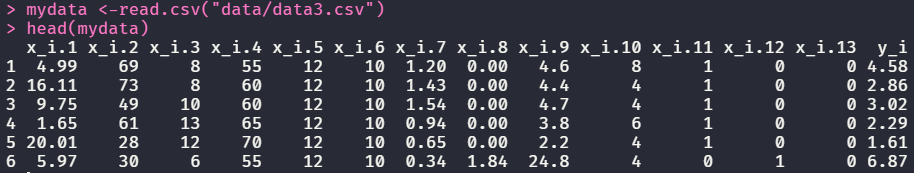
\includegraphics[width=0.8\linewidth]{images/B3/head-dataset}
	\caption{Một vài quan trắc đầu tiên}
	\label{fig-b3:head-dataset}
\end{figure}

Một số phân bố theo biến:
\begin{itemize}
	\item $X4$: Có 33 trong 39 quan trắc có tốc độ tối đa là 50, 55 và 60 (hình \ref{fig-b3:plot-x4}).
	\begin{figure}[H]
		\centering
		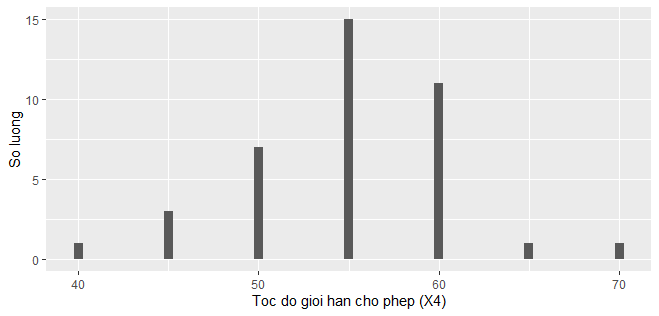
\includegraphics[width=0.7\linewidth]{images/B3/plot-x4}
		\caption{Phân bố theo tốc độ giới hạn cho phép ($X4$) (dặm/giờ)}
		\label{fig-b3:plot-x4}
	\end{figure}
	\item $X10$: Có 32 trong 39 quan trắc có tổng số làn đường là 2 hoặc 4 (hình \ref{fig-b3:plot-x10}).
		\begin{figure}[H]
			\centering
			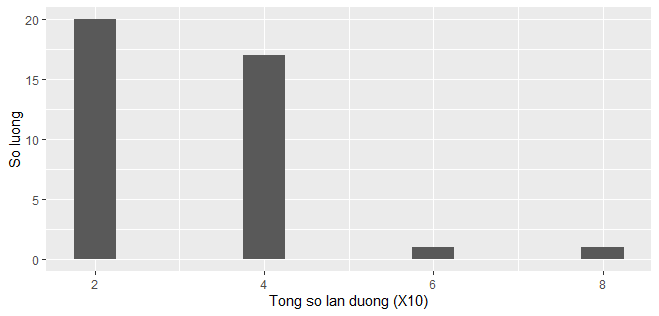
\includegraphics[width=0.7\linewidth]{images/B3/plot-x10}
			\caption{Phân bố theo tổng số làn đường ($X10$)}
			\label{fig-b3:plot-x10}
		\end{figure}
	\item $Y$: Phần lớn tỷ lệ \% tai nạn là $1-5\%$ (hình \ref{fig-b3:plot-y}).
		\begin{figure}[H]
			\centering
			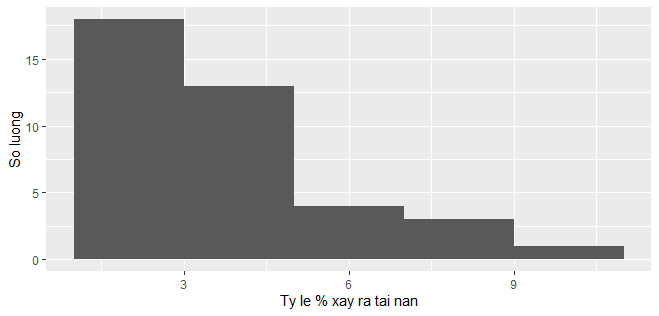
\includegraphics[width=0.7\linewidth]{images/B3/plot-y}
			\caption{Phân bố theo tỷ lệ \% tai nạn ($Y$)}
			\label{fig-b3:plot-y}
		\end{figure}
\end{itemize}

Trung bình của tổng tỷ lệ \% tai nạn theo các loại tuyến đường (hình \ref{fig-b3:aggregate-x11-13}) cho thấy loại tuyến đường cao tốc chính có tỷ lệ \% tai nạn cao nhất.
\begin{figure}[H]
	\centering
	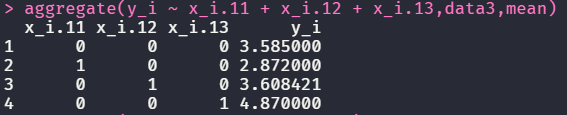
\includegraphics[width=0.7\linewidth]{images/B3/aggregate-x11-13}
	\caption{Trung bình của tổng tỷ lệ \% tai nạn theo các loại tuyến đường}
	\label{fig-b3:aggregate-x11-13}
\end{figure}

Trung bình của tổng tỷ lệ \% tai nạn theo các mức tốc độ giới hạn cho phép (hình \ref{fig-b3:aggregate-x4}) cho thấy giới hạn tốc độ cho phép trên đường cao tốc càng thấp thì xảy ra tai~nạn càng nhiều, tỷ lệ \% tai nạn giảm dần đều khi giới hạn tốc độ cho phép tăng.
\begin{figure}[H]
	\centering
	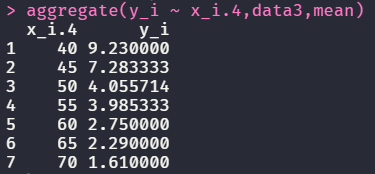
\includegraphics[width=0.45\linewidth]{images/B3/aggregate-x4}
	\caption{Trung bình của tổng tỷ lệ \% tai nạn theo các mức tốc độ giới hạn cho phép}
	\label{fig-b3:aggregate-x4}
\end{figure}

Trung bình của tổng tỷ lệ \% tai nạn theo tổng số làn đường (hình \ref{fig-b3:aggregate-x10}) cho thấy  trên đoạn đường có 8 làn đường có tỷ lệ \% tai nạn cao nhất, kế đến là đoạn đường có 2~làn.
\begin{figure}[H]
	\centering
	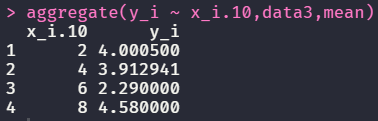
\includegraphics[width=0.45\linewidth]{images/B3/aggregate-x10}
	\caption{Trung bình của tổng tỷ lệ \% tai nạn theo tổng số làn đường}
	\label{fig-b3:aggregate-x10}
\end{figure}




\subsection*{Phân tích, chọn mô hình}
\subsection*{Kết luận}